\documentclass{standalone}
\usepackage{tikz}
\usepackage{mathrsfs}
\usetikzlibrary{shapes.geometric, arrows}
\tikzstyle{startstop} = [draw, rectangle, rounded corners, minimum width=3cm, minimum height=1cm,text centered, draw=black]
\tikzstyle{bola} = [draw, circle , minimum size = 10, draw=black, text centered]
\tikzstyle{elipse} = [draw, ellipse, minimum height = 10]
\begin{document}
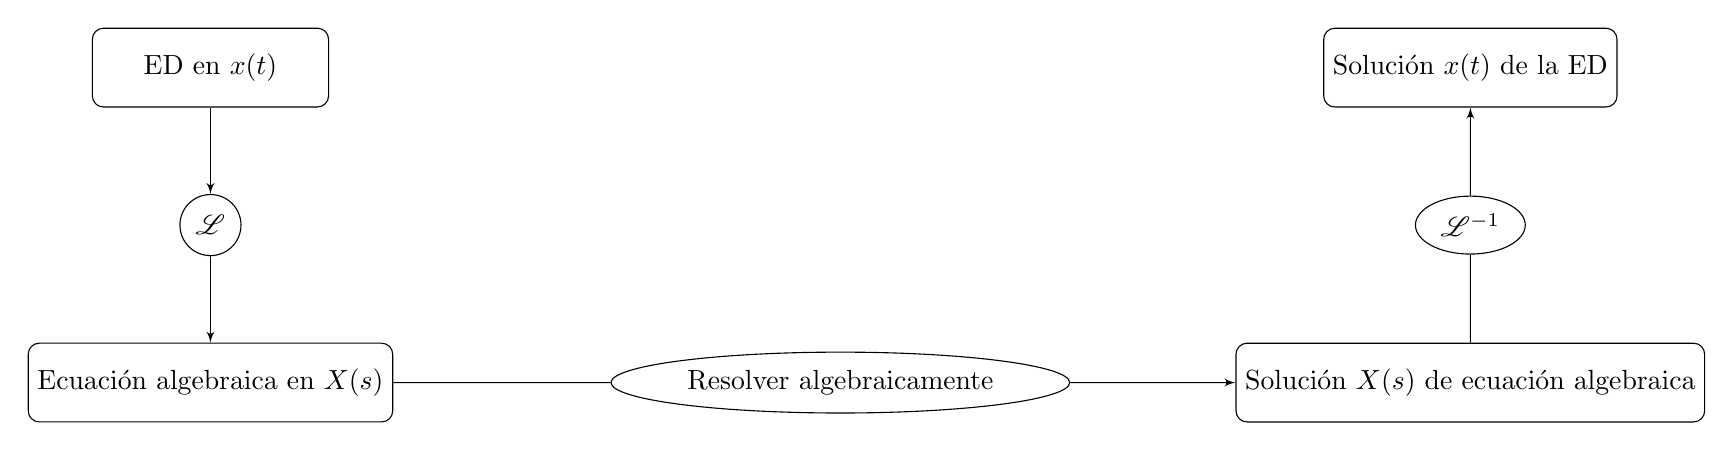
\begin{tikzpicture}[=>stealth, auto, node distance = 2cm, >=latex', scale=0.7]
\node (start) [startstop] {ED en $x(t)$};
\node (bola1) [bola, below of =start] {$\mathscr{L}$};
\node (start2) [startstop,below of = bola1] {Ecuaci\'{o}n algebraica en $X(s)$};
\node (elipse1) [elipse, right of = start2, node distance = 8cm] {Resolver algebraicamente};
\node (start3) [startstop, right of = elipse1, node distance = 8cm] {Soluci\'{o}n $X(s)$ de ecuaci\'{o}n algebraica};
\node (elipse2) [elipse, above of = start3] {$\mathscr{L}^{-1}$};
\node (start4) [startstop, above of = elipse2] {Soluci\'{o}n $x(t)$ de la ED};
\draw [->] (start) -- (bola1);
\draw [->] (bola1) -- (start2);
\draw (start2) -- (elipse1);
\draw [->] (elipse1) -- (start3);
\draw (start3) -- (elipse2);
\draw [->] (elipse2) -- (start4);

\end{tikzpicture}
\end{document}